\chapter{RESULTADOS Y DISCUSIÓN}
\label{sec:results_discussion}

En éste apartado se muestran los resultados obtenidos a partir de las pruebas experimentas, y las características más resaltantes que pudieron analizarse a partir de la serie de pruebas. 
\section{Ambiente de Pruebas experimentales}

El conjunto de pruebas se realizó sobre el siguiente hardware disponible: Una PC HP Proliant ML 110 Gen9 con las siguientes características:

\begin{itemize}
    \item Procesador Xeon E7 v3/Xeon E5 v3/Core i7,
    \item 8GB de memoria del sistema,
    \item Disco duro de 2TB MB2000GCWDA,
    \item Sistema Operativo CentOS 7 (centos-release-7-3.1611.el7.centos.x86\_64).
\end{itemize}


\section{Descripción de resultados obtenidos}

Se realizaron pruebas utilizando 8 imágenes a color a partir del conjunto de datos disponible en http://www.vision.caltech.edu/archive.html. La tabla \ref{table:parametrospso} muestra cómo $SMPSO$ fué configurada para la ejecución de prueba experimentales. Los detalles de implementación de $SMPSO$ está disponible en \cite{durillo2010jmetal}, mientras que los detalles de implementación para $CLAHE$, $\mathscr{H}$ y $SSIM$ están disponibles en \cite{bradski2000opencv}.

\begin{table}[H]
\setlength{\abovecaptionskip}{2pt plus 3pt minus 2pt} % Chosen fairly arbitrarily
\caption[Parámetros de entrada para $MOPSO$]{Parámetros de entrada iniciales para CMOPSO-CLAHE.}
\begin{center}
 \begin{tabular}{||c c | c c||} 
 \hline
 Parámetro & Valor & Parámetro & Valor \\ [0.5ex] 
 \hline\hline
 $L$ & $256$ &     &       \\ 
 \hline
 $M$ & $256$ & $N$ & $163$ \\ 
 \hline
 $lower\_limit_{\mathscr{R}_x}$ & $2$ & $upper\_limit_{\mathscr{R}_x}$ & $M/2$ \\ 
 \hline
 $lower\_limit_{\mathscr{R}_y}$ & $2$ & $upper\_limit_{\mathscr{R}_y}$ & $N/2$ \\  
 \hline
 $lower\_limit_{{\mathscr{C}}}$ & $0$ & $upper\_limit_{{\mathscr{C}}}$ & 0.5 \\
\hline
$\Omega$ & $100$ & $t_{max}$ & $100$ \\ 
\hline
$c_1$ $min$ & 1.5 & $c_1$ $max$ & 2.5 \\ 
\hline
$c_2$ $min$ & 1.5 & $c_2$ $max$ & 2.5 \\ 
\hline
$r_1$ $min$ & 0.0 & $r_1$ $max$ & 1.0 \\ 
\hline
$r_2$ $min$ & 0.0 & $r_2$ $max$ & 1.0 \\
\hline
\end{tabular}
\end{center}
\label{table:parametrospso}
\end{table}

Para cada imagen de prueba, se realizaron 50 ejecuciones, y en promedio se encontraron 100 soluciones no dominadas. De la Figura \ref{fig:casa1} se puede verificar que es notable la manera en que las variables de decisión entrenadas logran la Mejora del Contraste en las imágenes de prueba; además de que se puede evidenciar también la existencia una relación de compromiso con respecto a la variación de coeficientes entre $\mathscr{H}$ y $SSIM_R,SSIM_G,SSIM_B$. Es también notable a partir de la Figura (\ref{fig:casa1})(c) cómo los valores más altos de $\mathscr{H}$ degradan severamente a la imagen, mientras que los valores altos de $SSIM_R,SSIM_G,SSIM_B$ no logran el Contraste suficiente, en ocasiones siendo apenas perceptible; por lo que es necesario encontrar el balance correcto entre $\mathscr{H}$ y $SSIM_R,SSIM_G,SSIM_B$.

En el Anexo A se puede apreciar el detalle de coeficientes obtenidos para las métricas utilizadas en el trabajo.

%Tests were performed using 8 color images from the dataset available at http://www.vision.caltech.edu/archive.html. Table \ref{table:parametrospso} shows how $SMPSO$ was configured for the tests. $SMPSO$ implementation is available at \cite{durillo2010jmetal}, meanwhile the implementations for $CLAHE$, $\mathscr{H}$ and $SSIM$ are available at \cite{bradski2000opencv}. For every test image, 50 test were performed, and 10 non-dominated solutions were found in average. From Figures (\ref{fig:casa1original},\ref{fig:casa1enhanced1},\ref{fig:casa1enhanced2}) it is noticeable how CE is achieved; there is also a compromise relation between $\mathscr{H}$ and $SSIM_R,SSIM_G,SSIM_B$. It is noteworthy from Figure (\ref{fig:casa1enhanced2}) how higher values of $\mathscr{H}$ degrade images severely, so it is neccesary to find the correct balance between $\mathscr{H}$ and $SSIM_R,SSIM_G,SSIM_B$. In Figure (\ref{fig:casa1enhanced3}) it is shown the resultant image enhanced using the proposal described in \cite{morepso}; it is noticeable that the resultant image does not achieve good CE; this is because the mono-objective approach does not use color information properly, and this result is the same for other test images. In Table \ref{table:nodominadas}, the non-dominated metric coefficients are shown, and in the last line it is shown the metric coefficients for image (\ref{fig:casa1original}), enhanced using the mono-objective proposal. Although its metrics seem to fall in the Pareto Front, the visual information obtained is not enough to state that the mono-objective proposal is feasible for color images. These results are similar for every test image used.

% \begin{figure}[htp]

% \centering
% \includegraphics[width=.3\textwidth]{calhouse_0230.jpg}\hfill
% \includegraphics[width=.3\textwidth]{calhouse_0230_20-25165283474-10.jpg}\hfill
% 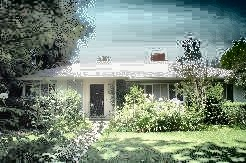
\includegraphics[width=.3\textwidth]{calhouse_0230_20-62968204656-00.jpg}

% \caption{default}
% \label{fig:figure3}

% \end{figure}

\begin{figure}[H]
    \centering
    %\begin{subfigure}[t]{0.45\textwidth}
    \begin{subfigure}[Imagen Original. $\mathscr{H_Y}=0.207231$, $SSIM_R=1$, $SSIM_G=1$, $SSIM_B=1$]{
        \includegraphics[width=0.45\textwidth]{./Figures/calhouse_0230.jpg}
    }
%        \caption{Imagen Original. $\mathscr{H_Y}=0.207231$, $SSIM_R=1$, $SSIM_G=1$, $SSIM_B=1$}
        \label{fig:casa1original}
    \end{subfigure}
    ~ %add desired spacing between images, e. g. ~, \quad, \qquad, \hfill etc. 
      %(or a blank line to force the subfigure onto a new line)
    \begin{subfigure}[Imagen mejorada. $\mathscr{H_Y}=0.611275$, $SSIM_R=0.00897331$, $SSIM_G=0.00823064$, $SSIM_B=0.00851013$]{
        \includegraphics[width=0.45\textwidth]{./Figures/calhouse_0230_20-25165283474-10.jpg}   
    }
    %\begin{subfigure}[t]{0.45\textwidth}
%        \caption{Enhanced Image. $\mathscr{H_Y}=0.611275$, $SSIM_R=0.00897331$, $SSIM_G=0.00823064$, $SSIM_B=0.00851013$}
        \label{fig:casa1enhanced1}
    \end{subfigure}
    ~ %add desired spacing between images, e. g. ~, \quad, \qquad, \hfill etc. 
    %(or a blank line to force the subfigure onto a new line)
    \begin{subfigure}[Imagen mejorada. $\mathscr{H_Y}=0.0350595$, $SSIM_R=0.416776$, $SSIM_G=0.403636$, $SSIM_B=0.417654$]{
        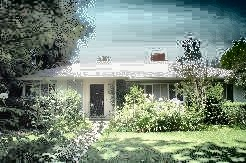
\includegraphics[width=0.45\textwidth]{calhouse_0230_20-62968204656-00.jpg}
    }
    % \begin{subfigure}[t]{0.45\textwidth}
%        \caption{Enhanced Image.  $\mathscr{H_Y}=0.0350595$, $SSIM_R=0.416776$, $SSIM_G=0.403636$, $SSIM_B=0.417654$}
        \label{fig:casa1enhanced2}
    \end{subfigure} 
    \begin{subfigure}[Imagen mejorada. $\mathscr{H_Y}=0.788927$, $SSIM_R=0.000204143$, $SSIM_G=0.0000526475$, $SSIM_B=0.0000518143$]{
        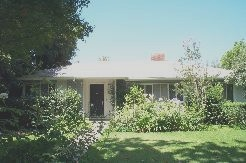
\includegraphics[width=0.45\textwidth]{calhouse_0230_20-20-0020072469292179818.jpg}
    }
    % \begin{subfigure}[t]{0.45\textwidth}
        % \caption{Enhanced Image using \cite{morepso}. $\mathscr{H_Y}=0.788927$, $SSIM_R=0.000204143$, $SSIM_G=0.0000526475$, $SSIM_B=0.0000518143$}
        \label{fig:casa1enhanced3}
    \end{subfigure}

    \caption{Imágenes original y resultantes para la imagen de prueba \texttt{calhouse\_230.jpg}}\label{fig:casa1}
\end{figure}


% \begin{table}[H]
% \setlength{\abovecaptionskip}{2pt plus 3pt minus 2pt} % Chosen fairly arbitrarily
% \caption[Parámetros de entrada para $MOPSO$]{Coeficientes de las métricas obtenidas utilizando CMOPSO-CLAHE para algunos resultados no dominados de la imagen en la Figura (\ref{fig:casa1}), además de los coeficientes obtenidos con el enfoque de \cite{morepso}, el cual se muestra en la última línea.}
% \begin{center}
% \resizebox{0.8\columnwidth}{!}{%
%  \begin{tabular}{||c | c c c c||} 
%  \hline
%  & $\mathscr{H_Y}$ & $SSIM_R$ & $SSIM_G$ & $SSIM_B$ \\ 
% \hline
% Result 1 & 0.544854	& 0.0155038	 & 0.0140995  & 0.0149364 \\ 
% \hline
% Result 2& 0.658577	& 0.00551113 & 0.00494194 & 0.00529456 \\ 
% \hline
% Result 3& 0.0425715	& 0.394656	 & 0.380667	  & 0.39842 \\ 
% \hline
% Result 4& 0.0365424	& 0.401675	 & 0.388628	  & 0.402692 \\ 
% \hline
% Result 5& 0.0350595	& 0.416776	 & 0.403636	  & 0.417654 \\ 
% \hline
% Result 6& 0.611275	& 0.00897331 & 0.00823064 & 0.00851013 \\ 
% \hline
% Result 7& 0.0342894	& 0.420948	 & 0.408035	  & 0.421891 \\ 
% \hline
% Result Mono& 0.788927    & 0.000204143 & 0.0000526475 & 0.0000518143 \\
% \hline
% \end{tabular}
% }
% \end{center}
% \label{table:nodominadas}
% \end{table}

\begin{table}[H]
\setlength{\abovecaptionskip}{2pt plus 3pt minus 2pt} % Chosen fairly arbitrarily
\caption[Parámetros de entrada para $MOPSO$]{Tabla de correlación entre métricas. Los datos fueron tomados de la Tabla de Anexo para la imagen \texttt{calhouse\_230.jpg}}
\begin{center}
 \begin{tabular}{||c | c c c c||} 
 \hline
Metrics & $\mathscr{H_Y}$ & $SSIM_R$ & $SSIM_G$ & $SSIM_B$ \\ 
\hline
$\mathscr{H_Y}$ & 1 &   &   &  \\ 
\hline
$SSIM_R$ & -0.9826  & 1 &  &  \\ 
\hline
$SSIM_G$ & -0.9823 & 0.9999   & 1   &  \\ 
\hline
$SSIM_B$ & -0.9826 & 0.9999   & 0.9999   & 1 \\ 
\hline
\end{tabular}
\end{center}
\label{table:correlacion}
\end{table}

\begin{figure}[H]
    \centering
        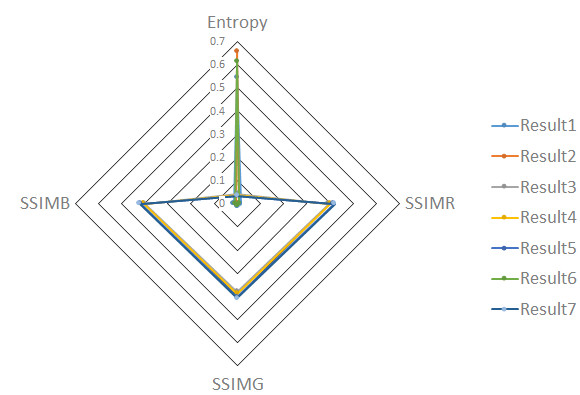
\includegraphics[width=0.80\textwidth]{./Figures/pareto_front.jpg}
    \caption{Frente Pareto dibujado utilizando datos de referencia métricas de la imagen de prueba \texttt{calhouse\_230.jpg} }\label{fig:pareto_front}
\end{figure}


La Figura (\ref{fig:pareto_front}) muestra el Frente pareto creado a partir de los datos de coeficientes de métricas de la imagen de prueba \texttt{calhouse\_230.jpg}, y también la Tabla \ref{table:correlacion} muestra la correlación entre métricas, analizadas a partir de los resultados de coeficientes de métricas de dicha imagen. Es notable cómo hay una correlación positiva muy fuerte entre $SSIM_R$, $SSIM_G$ y $SSIM_B$; también existe una correlación negativa entre las métricas previamente mencionadas y $\mathscr{H_Y}$. Éstas correlaciones indican que los canales  $R,G,B$ de las imágenes se ven afectadas directamente por el proceso que modifica el canal $Y$ (véase el Algoritmo (\ref{alg:pso_clahe})). Ésto también indica que la Mejora del Contraste de las imágenes a color se puede plantear como un problema de optimización bi-objetivo, utlizando simplemente $\mathscr{H_Y}$ y $SSIM$ aplicados sobre el canal $Y$, o posiblemente tomando como métrica de distorsión alguna métrica relacionada a la medición de variación de color.

Finalmente, se puede mencionar que los tiempos de ejecución de las pruebas (las cuales se detallan en el Anexo), muestran que es temporalmente factible realizar entrenamientos que posibilitan la obtención de variables de decisión adecuadas para el algoritmo de Mejora del Contraste, cuya aplicación posterior garantiza la posibilidad de resaltar distintos detalles de la imagen de acuerdo al contraste aplicado.

%Figure (\ref{fig:pareto_front}) shows the Pareto Front created from the data in Table \ref{table:nodominadas}, and also Table \ref{table:correlacion} shows the correlation between metrics, analized from the results in Table \ref{table:nodominadas}. It is remarkable that there is a strong positive correlation between $SSIM_R$, $SSIM_G$ and $SSIM_B$; and there is a negative correlation between the previously mentioned metrics and $\mathscr{H_Y}$. These correlations indicate that the channels $R,G,B$ of images are directly affected by the proccess that modifies $Y$ channel (see Algorithm (\ref{alg:pso_clahe})). This also indicates that CE of color images can be posed as a bi-objective optimization problem, using only $\mathscr{H_Y}$ and $SSIM$ applied over $Y$ channel.

% En este apartado se exponen los resultados experimentales para las imágenes en escala de grises y las imágenes en color, además de las métricas de mejora del contraste utilizados para medir la calidad de la imagen resultante. La cuantificación de la mejora del contraste es difícil, no existe una medida específica que mide el rendimiento del algoritmo de mejora \cite{gordon1984feature,wang2003chromosome}.

% Para la comparación se utilizan algoritmos de mejora de contraste que modifican el histograma, los cuales son \textit{Histogram Equalization} (HE) \cite{huang2006natural} \label{symbol:he} que realiza una mejora global, \textit{Contrast-Limited Adaptive Histogram Equalization} (CLAHE) \label{symbol:clahe} \cite{zuiderveld1994contrast} que realiza una mejora local. También se comparó con el algoritmo MMCE\label{symbol:mmce} que utiliza la transformada de top-hat en escalas múltiples. Los algoritmos HE y CLAHE fueron seleccionados para la comparación porque se utilizaron en la propuesta de Bai. et. al. \cite{bai2012image}. Y se comparó con el algoritmo MMCE porque fue el que modificamos en este trabajo.

% Para el experimento se utilizaron 200 diferentes imágenes en color de una base de datos pública \cite{arbelaez2007berkeley}. El tamaño de las imágenes en color son de $481 \times 321$ y de $321 \times 481$. Los algoritmos propuesto y MMCE se ejecutaron en un ordenador que posee un procesador Intel Core i5-4570 de doble núcleo con una velocidad de 3.20GHz, una memoria RAM de 8GB, un disco duro de 1TB. El sistema operativo del ordenador es Windows 8.1 pro de 64 bits. 

% \section{Experimento 1 - Imágenes en escala de grises}

% En este apartado se muestra el experimento realizado con imágenes en escala de grises. Para validar las mejoras en la imagen se utilizaron dos métricas; una que evalúa la mejora del contraste global y otra que evalúa la mejora del contraste local. 

% \subsection{Métricas de evaluación}
% %La métrica \textit{Contrast} (C)\label{symbol:cf}\cite{moulden1990standard} se utilizó para cuantificar la mejora del contraste global en imágenes en escala de grises, se define como:
% La métrica \textit{Contrast} (C)\label{symbol:cf}\cite{moulden1990standard} se utilizó para cuantificar el contraste global de las imágenes en escala de grises, se define como:

% \begin{equation}
% \label{contraste}
% C(f) = \sqrt{\sum_{j=0}^{L-1}(j-E(f))^{2}\times P(j)},
% \end{equation}
% donde $j$ representa el valor del píxel $(u,v)$ de la imagen $f$, $L$ son los niveles de grises, $E(f)$\label{symbol:E} representa la intensidad media de la imagen y $P(j)$\label{symbol:P} es la probabilidad de ocurrencia del valor $j$. El valor $C(f_{E})$ de la imagen resultante debe ser mayor al valor $C(f)$ de la imagen original para suponer mejora.
% %El valor $C(f)$ de la imagen resultante debe ser mayor al de la imagen original para suponer mejora.

% La métrica adoptada para evaluar la mejora del contraste local de la imagen en escala de grises se denomina \textit{Contrast Improvement Ratio} (CIR)\label{symbol:cir}.

% El contraste local se define como la diferencia de los valores medios en dos ventanas rectangulares centradas en un píxel \cite{gordon1984feature}. Específicamente, el contraste local $\omega(u,v)$ se define como:

% \begin{equation}
% \label{lc}
% \omega(u,v) = \dfrac{|\rho - \iota|}{|\rho + \iota|},
% \end{equation}
% donde $\rho$\label{rho} y $\iota$\label{iota} son los valores de los niveles de grises del píxel central y la media del los vecinos dentro de una ventana de $3 \times 3$. Da la medida de contraste en el rango [0,1].

% El CIR se define como la relación de la imagen mejorada y la imagen original dentro de la región de interés $f$, es decir \cite{wang2003chromosome}:

% \begin{equation}
% \label{symbol:cir1}
% CIR(f,f_{E}) = \dfrac{\sum_{(u,v)\in D}{| \omega(u,v) - \tilde{\omega}(u,v) |^{2} }}{\sum_{(u,v)\in D } {\omega(u,v)^{2} }},
% \end{equation}
% donde $\omega$ y $\tilde{\omega}$\label{lct} son los valores de contraste locales de las imágenes original y realzada, respectivamente. En nuestros experimentos, asumimos que $f$ es toda la imagen y $D$\label{D} es todo su dominio.

% \subsection{Resultados experimentales}

% Las 200 imágenes en color se convirtieron en imágenes en escala de grises de 8 bits utilizando el framework ImageJ \cite{schneider2012nih}. Dentro del experimento los valores para los algoritmos HE y CLAHE fueron por defecto. Las pruebas con estos algoritmos se realizaron con el programa MATLAB \cite{zuiderveld1994contrast}. Los algoritmos MMCE y el propuesto fueron implementados con el framework ImageJ \cite{schneider2012nih}, los parámetros de entrada fueron la imagen original en escala de grises $f$, el número de iteraciones $n=7$ y el elemento estructurante inicial $g_{1}$ cuadrado de $3\times 3$. 

% En la Figura \ref{f:I4} se muestra (a) la imagen original \textit{164046}, (b) la imagen mejorada con el algoritmo HE, (c) la imagen mejorada con el algoritmo CLAHE, (d) la imagen mejorada con el algoritmo MMCE y (e) la imagen mejorada con el algoritmo propuesto. Los algoritmos HE, CLAHE, MMCE y el propuesto mejoran el contraste de las imágenes en escala de grises. El aporte de la mejora númerica del algoritmo propuesto se puede notar en las evaluaciones de las imágenes realizadas con las métricas utilizadas.

% \begin{figure}[H]
% 	\centering
% 	\subfigure[]{\includegraphics[width = 1.72in]{./Figures/164046_OG.jpg}}
% 	\subfigure[]{\includegraphics[width = 1.72in]{./Figures/164046_HE.jpg}}
% 	\subfigure[]{\includegraphics[width = 1.72in]{./Figures/164046_CLAHE.jpg}}
% 	\subfigure[]{\includegraphics[width = 1.72in]{./Figures/164046_AC_G.jpg}}
% 	\subfigure[]{\includegraphics[width = 1.72in]{./Figures/164046_AP_G.jpg}}
% 	\caption{(a) Imagen original \textit{164046} en escala de grises, (b) imagen mejorada con el algoritmo  HE, (c) imagen mejorada con el algoritmo  CLAHE, (d) imagen mejorada con el algoritmo  MMCE y (e) imagen mejorada con el algoritmo  propuesto.}
% 	\label{f:I4}
% \end{figure}

% En las Figuras \ref{f:I21}, \ref{f:I22} se muestran el zoom de la imagen en escala de grises mejorada con el algoritmo MMCE y el zoom de la imagen en escala de grises mejorada con el algoritmo propuesto. La diferencia visual entre las figuras es que la imagen mejorada con el algoritmo propuesto presenta una mejor diferenciación de los detalles oscuros y claros de la imagen.

% \begin{figure}[!ht]
% 	\centering
% 	\begin{tikzpicture}[spy using outlines={circle,yellow,magnification=5,size=5cm, connect spies}]
% 	\node {\pgfimage[width=0.32\textwidth]{./Figures/164046_AC_G.jpg}};
% 	\spy on (0,0.4) in node [left] at (10,1.25);
% 	\end{tikzpicture}
% 	\caption{Zoom de la imagen en escala de grises mejorada con el algoritmo MMCE.}
% 	\label{f:I21}
% \end{figure}

% \begin{figure}[!ht]
% 	\centering
% 	\begin{tikzpicture}[spy using outlines={circle,yellow,magnification=5,size=5cm, connect spies}]
% 	\node {\pgfimage[width=0.32\textwidth]{./Figures/164046_AP_G.jpg}};
% 	\spy on (0,0.4) in node [left] at (10,1.25);
% 	\end{tikzpicture}
% 	\caption{Zoom de la imagen en escala de grises mejorada con el algoritmo propuesto.}
% 	\label{f:I22}
% \end{figure}

% En la Tabla \ref{tabla01} se puede observar la cuantificación de la mejora de contraste de acuerdo con las métricas C y CIR para imágenes en escala de grises. Además se muestran las desviaciones típicas $\sigma$ de los algoritmos. La imagen original $f$ tiene $C=50,856$ y $\sigma = \pm 13,913$.

% \begin{table}[H]
% \centering
% \caption{Promedio de las 200 imágenes con mejora de contraste de acuerdo con las métricas C y CIR para imágenes en escala de grises.}
% \label{tabla01}
% \begin{tabular}{|c|cc|cc|cc|cc|}
% \hline
% Mét. & \multicolumn{1}{c|}{HE} & $\sigma$($\pm$)             & \multicolumn{1}{c|}{CLAHE} & $\sigma$($\pm$)             & \multicolumn{1}{c|}{MMCE} & $\sigma$($\pm$)     & \multicolumn{1}{c|}{Prop.} & $\sigma$($\pm$)     \\ \hline
% C        & 74,919                  & \textbf{1,029} & 62,458                     & 8,059          & 70,462                    & 14,023 & \textbf{76,124}                & 13,706 \\
% CIR      & 5,117                   & 5,490          & 2,106                      & \textbf{1,626} & 14,011                    & 7,088  & \textbf{22,066}                & 12,304 \\ \hline
% \end{tabular}
% \end{table}

% % \begin{table}[!ht]
% % 	\centering
% % 	\caption{Promedio de las 200 imágenes con mejora de contraste de acuerdo con las métricas C y CIR para imágenes en escala de grises.}
% % 	\label{tabla01}
% % 	\begin{tabular}{|l|rrrr|}
% % 		\multicolumn{5}{l}{} \\
% % 		\hline
% % 		Métricas	&	HE				&	CLAHE			&	MMCE			&	Propuesta\\
% % 		\hline
% % 		C			&	74,919			&	62,458			&	70,462 			& 	\textbf{76,124}\\
% % 		CIR			&	5,117			&	2,106			&	14,011 			& 	\textbf{22,066}\\
% % 		\hline
% % 	\end{tabular}
% % \end{table}

% En la Tabla \ref{tabla06} se puede observar los promedios obtenidos por cada iteración de los algoritmos MMCE y el propuesto, teniendo en cuenta la métrica C para las imágenes en escala de grises. Además se muestran las desviaciones típicas $\sigma$($\pm$) de los algoritmos para la métrica C por cada iteración y los porcentajes de mejoras con respecto a la imagen original. La imagen original $f$ tiene $C=50,856$ y $\sigma = \pm 13,913$.

% % Please add the following required packages to your document preamble:
% % \usepackage{multirow}
% \begin{table}[H]
% \centering
% \caption{Promedios obtenidos por cada iteración de los algoritmos MMCE y el propuesto, teniendo en cuenta la métrica C para las imágenes en escala de grises}
% \label{tabla06}
% \begin{tabular}{|c|ccc|ccc|c|}
% \hline
% \multirow{2}{*}{Iter. (n)} & \multicolumn{3}{c|}{MMCE}                                 & \multicolumn{3}{c|}{Propuesta}                            & \multirow{2}{*}{\begin{tabular}[c]{@{}c@{}}\% de \\ ganancia\end{tabular}} \\ \cline{2-7}
%                            & \multicolumn{1}{c|}{C} & \multicolumn{1}{c|}{$\sigma$($\pm$)} & \%     & \multicolumn{1}{c|}{C} & \multicolumn{1}{c|}{$\sigma$($\pm$)} & \%     &                                                                            \\ \hline
% 1                          & 56,758                 & 13,649                  & 12,964 & 56,758                 & 13,649                  & 12,964 & 0                                                                          \\
% 2                          & 63,984                 & 13,615                  & 29,001 & 63,984                 & 13,615                  & 29,001 & 0                                                                          \\
% 3                          & 65,529                 & 13,694                  & 32,292 & 69,371                 & 13,739                  & 40,944 & 8,652                                                                      \\
% 4                          & 67,014                 & 13,788                  & 35,435 & 69,634                 & 13,720                  & 41,373 & 5,938                                                                      \\
% 5                          & 68,286                 & 13,845                  & 38,123 & 73,354                 & 13,720                  & 49,592 & 11,470                                                                     \\
% 6                          & 69,469                 & 13,976                  & 40,587 & 73,224                 & 13,800                  & 49,104 & 8,517                                                                      \\
% 7                          & 70,462                 & 14,023                  & 42,655 & 76,124                 & 13,706                  & 55,512 & 12,857                                                                     \\ \hline
% Promedio                   & 65,929                 & 13,799                  & 33,008 & \textbf{68,921}                 & \textbf{13,707}                  & \textbf{39,784} & \textbf{6,776}                                                                      \\ \hline
% \end{tabular}
% \end{table}

% En la Tabla \ref{tabla07} se puede observar los promedios obtenidos por cada iteración de los algoritmos MMCE y el propuesto, teniendo en cuenta la métrica CIR para las imágenes en escala de grises. Además se muestran las desviaciones típicas $\sigma$($\pm$) de la métrica CIR de los algoritmos.

% % Please add the following required packages to your document preamble:
% % \usepackage{multirow}
% \begin{table}[H]
% \centering
% \caption{Promedios obtenidos por cada iteración de los algoritmos MMCE y el propuesto, teniendo en cuenta la métrica CIR para las imágenes en escala de grises.}
% \label{tabla07}
% \begin{tabular}{|c|cc|cc|}
% \hline
% \multirow{2}{*}{Iter.(n)} & \multicolumn{2}{c|}{MMCE}                 & \multicolumn{2}{c|}{Propuesta}    \\ \cline{2-5} 
%                           & \multicolumn{1}{c|}{CIR} & $\sigma$($\pm$)             & \multicolumn{1}{c|}{CIR} & $\sigma$($\pm$)     \\ \hline
% 1                         & 2,374                    & 0,590          & 2,374                    & 0,590  \\
% 2                         & 8,145                    & 2,907          & 8,145                    & 2,907  \\
% 3                         & 9,369                    & 3,712          & 14,611                   & 6,165  \\
% 4                         & 10,662                   & 4,538          & 13,730                   & 6,423  \\
% 5                         & 11,870                   & 5,421          & 19,035                   & 9,542  \\
% 6                         & 13,009                   & 6,254          & 17,352                   & 9,370  \\
% 7                         & 14,011                   & 7,088          & 22,066                   & 12,304 \\ \hline
% Promedio                  & 9,920                    & \textbf{4,359} & \textbf{13,902}          & 6,757  \\ \hline
% \end{tabular}
% \end{table}

% % \begin{table}[H]
% % 	\centering
% % 	\caption{Promedios obtenidos por cada iteración de los algoritmos MMCE y el propuesto, teniendo en cuenta la métrica CIR para las imágenes en escala de grises.}
% % 	\label{tabla07}
% % 	\begin{tabular}{|l|rrrrrrr|}
% % 		\multicolumn{8}{l}{} \\
% % 		\hline
% % 		Iter.(n)	&	1		&	2			&	3			&	4			&	5			&	6			&	7\\
% % 		\hline
% % 		MMCE		&	2,374	&	8,145		&	9,369		&	10,662		&	11,870		&	13,009		&	14,011\\
% % 		Propuesta	&	2,374	&	8,145		&	\textbf{14,611}		&	\textbf{13,730}		&	\textbf{19,035}		&	\textbf{17,352}		&	\textbf{22,066}\\
% % 		\hline
% % 	\end{tabular}
% % \end{table}

% %%%%%%%%%%%%%%%%%%%%%%%%%%%%%%%%%%%%%%%%%%%%%%%%%%%%%%%%%%%%%%%%%%%%%%%%%%%%
% %Agregar el tiempo de computo por cada iteracion, agregar la discusion
% %%%%%%%%%%%%%%%%%%%%%%%%%%%%%%%%%%%%%%%%%%%%%%%%%%%%%%%%%%%%%%%%%%%%%%%%%%%%

% En la Tabla \ref{tabla16} se puede observar los promedios de los tiempos (t), medidos en milisegundos (ms), de procesamiento de cada imagen en escala de grises para cada iteración. Éstos tiempos son para los algoritmos propuesto y MMCE. Para la medición de los tiempos de ejecución los algoritmos multiescala se ejecutaron 5 veces para las 200 imágenes por cada iteración. 

% % Please add the following required packages to your document preamble:
% % \usepackage{multirow}
% \begin{table}[H]
% \centering
% \caption{Promedios de los tiempos de procesamiento de las imágenes en escala de grises para cada iteración.}
% \label{tabla16}
% \begin{tabular}{|c|c|c|}
% \hline
% \multirow{2}{*}{Iter. (n)} & MMCE  & Propuesta \\ \cline{2-3} 
%                            & t(ms) & t(ms)     \\ \hline
% 1                          & 63    & 63        \\
% 2                          & 170   & 169       \\
% 3                          & 332   & 331       \\
% 4                          & 570   & 572       \\
% 5                          & 977   & 973       \\
% 6                          & 1458  & 1465      \\
% 7                          & 2036  & 2043      \\ \hline
% \end{tabular}
% \end{table}

% %%%%%%%%%%%%%%%%%%%%%%%%%%%%%%%%%%%%%%%%%%%%%%%%%%%%%%%%%%%%%%%%%%%%%%%%%%%%
% %El tiempo de procesamiento de las imágenes en escala de grises obtenidos por el algoritmo HE es $0,35$ ms y por el algortimo CLAHE es $595$ ms.
% %%%%%%%%%%%%%%%%%%%%%%%%%%%%%%%%%%%%%%%%%%%%%%%%%%%%%%%%%%%%%%%%%%%%%%%%%%%%

% \subsection{Discusión}

% En las imágenes en escala de grises con mejora de contraste, visualmente podemos observar que los algoritmos de multiescala distribuyen la intensidad de brillo en forma más homogénea que los algoritmos clásicos.

% En promedio para la métrica C, el algoritmo propuesto mejora en un $6,776$\% las imágenes en escala de grises con respecto al algoritmo MMCE. Además para $n=7$ supera numéricamente al algoritmo HE y para $n=2$ supera numéricamente al algoritmo CLAHE. En promedio la desviación típica obtenida por el algoritmo propuesto para la métrica C es menor que la obtenida por el algoritmo MMCE.

% Para la métrica CIR, el algoritmo propuesto obtuvo en la 3ra iteración similares resultados al que obtuvo el algoritmo MMCE en la 7ma iteración para las imágenes en escala de grises. Para $n=2$ el algoritmo propuesto obtuvo mejores resultados que los algoritmos HE y CLAHE. En promedio la desviación típica obtenida por el algoritmo propuesto para la métrica CIR es mayor que la obtenida por el algoritmo MMCE.

% Los tiempos de ejecución de los algoritmos multiescala para cada iteración son muy similares. Si el algoritmo propuesto obtiene mejores resultados en menos iteraciones con respecto al algoritmo MMCE, entonces podemos decir que el tiempo de procesamiento de las imágenes en escala de grises de la propuesta es mejor.

% El algoritmo propuesto mejora las imágenes en escala de grises local y globálmente. El algoritmo propuesto y el algoritmo MMCE arrojan los mismos resultados para las iteraciones 1 y 2. Para resaltar los mejores resultados numéricos se muestran en negrita. A partir de la 3ra iteración el algoritmo propuesto con respecto al algoritmo MMCE da mejores resultados numéricos para las imágenes en escala de grises. 

% \section{Experimento 2 - imágenes en color}

% A continuación se listan los códigos utilizados para abreviar los nombres de los métodos de ordenamiento que fueron objeto de experimentación:
% \begin{itemize}
% 	\item TPSA: Se utiliza el ordenamiento total en RGB para ordenar los colores.
% 	\item JLVN: Se utiliza el ordenamiento lexicográfico $T\longrightarrow R\longrightarrow G \longrightarrow B$ en RGB para ordenar los colores.
% 	\item IHS: Se utiliza el ordenamiento lexicográfico $I\longrightarrow H\longrightarrow S$ en HSI para ordenar los colores.
% 	\item VHS: Se utiliza el ordenamiento lexicográfico $V\longrightarrow H\longrightarrow S$ en HSV para ordenar los colores.
% \end{itemize}

% En el experimento 2 se muestran los resultados obtenidos para las imágenes en color. Para validar las mejoras en la imagen se utilizaron dos métricas. Uno que evalúa la mejora del contraste global y otro que evalúa la mejora del contraste local. 

% \subsection{Métricas de evaluación}
% La métrica que se utilizó para evaluar la mejora del color global de una imagen se denomina \textit{Color Enhancement Factor}. Esta métrica cuantifica el nivel de la mejora del color de una imagen como se menciona en \cite{susstrunk2003color}, aplicado a la imagen $f$ esta basado en la media y la desviación estándar de dos ejes de una sencilla representación de color contrario con $\gamma = f_{1} - f_{2}$\label{symbol:gamma} y $\beta = \dfrac{1}{2}(f_{1} + f_{2}) - f_{3}$\label{symbol:beta}, donde $f_{1}$ representa el canal $R$, $f_{2}$ representa el canal $G$ y $f_{3}$ representa el canal $B$ del espacio de color RGB. La ecuación \ref{symbol:cm} representa el nivel del color de la imagen $f$ de la siguiente forma:
% \begin{equation}
% \label{symbol:cm}
% CM(f) = \sqrt{\sigma_{\gamma}^{2} + \sigma_{\beta}^{2}} + 0.3\sqrt{\mu_{\gamma}^{2} + \mu_{\beta}^{2}},
% \end{equation}
% donde $\sigma_{\gamma}$ y $\sigma_{\beta}$ corresponden a la desviación estándar de $\gamma$ y $\beta$ respectivamente. De manera similar, $\mu_{\gamma}$ y $\mu_{\beta}$ corresponde a la media respectivamente.

% Entonces el $CEF$ se calcula por medio del cociente entre los valores de $CM(f_{E})$ y $CM(f)$:

% \begin{equation}
% \label{symbol:cef}
% CEF(f,f_{E}) = \dfrac{CM(f_{E})}{CM(f)},
% \end{equation}
% donde $CM(f_{E})$ es el valor obtenido de la imagen contrastada $f_{E}$ producto de aplicar la ecuación \ref{symbol:cm} y $CM(f)$ representa el resultado de aplicar la ecuación \ref{symbol:cm} a la imagen original $f$. Si el resultado del cociente es mayor a uno, entonces la métrica de la ecuación \ref{symbol:cef} indica una mejora del color global, de lo contrario no hay una mejora.

% En el experimento anterior \textit{CIR} se adopto para evaluar la mejora del contraste local de las imágenes en escala de grises. Para su aplicación en imágenes en color se realiza promediando el CIR de los canales RGB de la imagen. Es decir: 

% \begin{equation}
% \label{symbol:cirr}
% CIR_{RGB}(f,f_{E}) = \dfrac{CIR_R + CIR_G + CIR_B}{3}.
% \end{equation}

% \subsection{Resultados experimentales}

% Para de los algoritmos HE y CLAHE se aplicaron a las imágenes en color de manera marginal. Estos algoritmos fueron implementados en MATLAB \cite{zuiderveld1994contrast}. Los algoritmos MMCE y el propuesto fueron implementados en con framework ImageJ \cite{schneider2012nih}. Los parámetros de entrada fueron la imagen original en color $f$, el número de iteraciones $n=7$ y el elemento estructurante inicial $g$ cuadrado de $3\times 3$. 

% En la Figura \ref{f:I15} se muestran (a) la imagen original \textit{49024} en color, (b) la imagen mejorada con el algoritmo HE, (c) la imagen mejorada con el algoritmo CLAHE, (d) la imagen mejorada con el algoritmo MMCE y (e) la imagen mejorada con el algoritmo propuesto.

% \begin{figure}[H]
% 	\centering
% 	\subfigure[]{\includegraphics[width = 2.5in]{./Figures/49024_C.jpg}}
% 	\subfigure[]{\includegraphics[width = 2.5in]{./Figures/49024_HE_C.jpg}}
% 	\subfigure[]{\includegraphics[width = 2.5in]{./Figures/49024_CLAHE_C.jpg}}
% 	\subfigure[]{\includegraphics[width = 2.5in]{./Figures/49024_AC_TRGB.jpg}}
% 	\subfigure[]{\includegraphics[width = 2.5in]{./Figures/49024_AP_TRGB.jpg}}
% 	\caption{(a) Imagen \textit{49024} en color, (b) imagen mejorada con el algoritmo HE de manera marginal, (c) imagen mejorada con el algoritmo CLAHE de manera marginal, (d) imagen mejorada con el algoritmo MMCE con orden JLVN y (e) imagen mejorada con el algoritmo propuesto con orden JLVN.}
% 	\label{f:I15}
% \end{figure}


% % \begin{table}[!ht]
% % 	\centering
% % 	\caption{Promedio de las 200 imágenes en color con mejora de contraste de acuerdo con las métricas CEF y CIR y el orden JLVN.}
% % 	\label{tabla02}
% % 	\begin{tabular}{|l|rrrr|}
% % 		\multicolumn{5}{l}{} \\
% % 		\hline
% % 		Métricas	&	HE				&	CLAHE			&	MMCE			&	Propuesta\\
% % 		\hline
% % 		CEF			&	1,426			&	1,049			&	1,268			& 	\textbf{1,512}\\
% % 		CIR			&	5,151			&	2,381			&	11,742		 	& 	\textbf{24,084}	\\
% % 		\hline	
% % 	\end{tabular}
% % \end{table}

% En la Tabla \ref{tabla08} se puede observar los promedios obtenidos por cada iteración de los algoritmos propuesto y MMCE, teniendo en cuenta la métrica CEF y los ordenamientos para las imágenes en color.

% %%%%%%%%%%%%%%%%%%%%%%%%%%%%%%%%%%%%%%%%%%%%%%%%%%%%%%%%%%%%%%%%%%%%%%%%%%%%%%%%%%%%%%%%%%%%%%%%%%%%%%%%%%%%%%%%%%%%%%%%%%%%%%%%%
% % Please add the following required packages to your document preamble:
% % \usepackage{multirow}
% \begin{table}[H]
% \centering
% \caption{Promedios obtenidos por cada iteración de los algoritmos propuesto y MMCE, teniendo en cuenta la métrica CEF}
% \label{tabla08}
% \begin{tabular}{|c|cccc|cccc|}
% \hline
% \multirow{3}{*}{Iter. (n)}     & \multicolumn{4}{c|}{MMCE}                                                                                      & \multicolumn{4}{c|}{Propuesta}                                                                                                                     \\ \cline{2-9} 
%                                & \multicolumn{1}{c|}{JLVN} & \multicolumn{1}{c|}{TPSA} & \multicolumn{1}{c|}{IHS}  & VHS                        & \multicolumn{1}{c|}{JLVN}          & \multicolumn{1}{c|}{TPSA}          & \multicolumn{1}{c|}{IHS}           & VHS                                 \\ \cline{2-9} 
%                                & \multicolumn{1}{c|}{CEF}  & \multicolumn{1}{c|}{CEF}  & \multicolumn{1}{c|}{CEF}  & CEF                        & \multicolumn{1}{c|}{CEF}           & \multicolumn{1}{c|}{CEF}           & \multicolumn{1}{c|}{CEF}           & CEF                                 \\ \hline
% 1                              & 1,019                     & 1,019                     & 1,046                     & 1,031                      & 1,019                              & 1,019                              & 1,046                              & 1,031                               \\
% 2                              & 1,065                     & 1,065                     & 1,101                     & 1,085                      & 1,065                              & 1,065                              & 1,101                              & 1,085                               \\
% 3                              & 1,112                     & 1,111                     & 1,157                     & 1,139                      & 1,255                              & 1,252                              & 1,344                              & 1,311                               \\
% 4                              & 1,158                     & 1,155                     & 1,208                     & 1,192                      & 1,335                              & 1,330                              & 1,430                              & 1,401                               \\
% 5                              & 1,198                     & 1,191                     & 1,250                     & 1,237                      & 1,402                              & 1,388                              & 1,495                              & 1,472                               \\
% 6                              & 1,235                     & 1,225                     & 1,288                     & 1,279                      & 1,464                              & 1,448                              & 1,557                              & 1,543                               \\
% 7                              & 1,268                     & 1,257                     & 1,321                     & 1,315                      & 1,512                              & 1,496                              & 1,605                              & 1,593                               \\ \hline
% \multicolumn{1}{|l|}{Promedio} & \multicolumn{1}{l}{1,151} & \multicolumn{1}{l}{1,146} & \multicolumn{1}{l}{1,196} & \multicolumn{1}{l|}{1,183} & \multicolumn{1}{l}{\textbf{1,293}} & \multicolumn{1}{l}{\textbf{1,285}} & \multicolumn{1}{l}{\textbf{1,368}} & \multicolumn{1}{l|}{\textbf{1,348}} \\ \hline
% \end{tabular}
% \end{table}
% %%%%%%%%%%%%%%%%%%%%%%%%%%%%%%%%%%%%%%%%%%%%%%%%%%%%%%%%%%%%%%%%%%%%%%%%%%%%%%%%%%%%%%%%%%%%%%%%%%%%%%%%%%%%%%%%%%%%%%%%%%%%%%%%%

% % \begin{table}[!ht]
% % 	\centering
% % 	\caption{Promedios obtenidos por cada iteración de los algoritmos MMCE y el propuesto, teniendo en cuenta la métrica CEF y el orden JLVN para las imágenes en color.}
% % 	\label{tabla08}
% % 	\begin{tabular}{|l|rrrrrrr|}
% % 		\multicolumn{8}{l}{} \\
% % 		\hline
% % 		Iter.(n)	&	1		&	2			&	3			&	4			&	5			&	6			&	7\\
% % 		\hline
% % 		MMCE		&	1,0192	&	1,0652		&	1,112		&	1,158		&	1,198		&	1,235		&	1,268\\
% % 		Propuesta	&	1,0192	&	1,0652		&	\textbf{1,255}		&	\textbf{1,335}		&	\textbf{1,402}		&	\textbf{1,464}		&	\textbf{1,512}\\
% % 		\hline
% % 	\end{tabular}
% % \end{table}

% En la Figura \ref{f:I16} se muestran (a) la imagen original \textit{164046} en color, (c) la imagen mejorada con el algoritmo MMCE y (d) la imagen mejorada con el algoritmo propuesto.

% \begin{figure}[H]
% 	\centering
% 	\subfigure[]{\includegraphics[width = 1.72in]{./Figures/164046.jpg}}
% 	\subfigure[]{\includegraphics[width = 1.72in]{./Figures/164046_AC_RGB.jpg}}
% 	\subfigure[]{\includegraphics[width = 1.72in]{./Figures/164046_AP_RGB.jpg}}
% 	\caption{(a) Imagen \textit{164046} en color, (b) imagen mejorada con el algoritmo MMCE con orden TPSA y (c) imagen mejorada con el algoritmo propuesto con orden TPSA.}
% 	\label{f:I16}
% \end{figure}

% En la Tabla \ref{tabla09} se puede observar los promedios obtenidos por cada iteración de los algoritmos propuesto y MMCE, teniendo en cuenta la métrica CIR y los ordenamientos para las imágenes en color.

% %%%%%%%%%%%%%%%%%%%%%%%%%%%%%%%%%%%%%%%%%%%%%%%%%%%%%%%%%%%%%%%%%%%%%%%%%%%%%%%%%%%%%%%%%%%%%%%%%%%%%%%%%%%%%%%%%%%%%%%%%%%%%%
% % Please add the following required packages to your document preamble:
% % \usepackage{multirow}
% \begin{table}[H]
% \centering
% \caption{Promedios obtenidos por cada iteración de los algoritmos propuesto y MMCE, teniendo en cuenta la métrica CIR}
% \label{tabla09}
% \begin{tabular}{|c|cccc|cccc|}
% \hline
% \multirow{3}{*}{Iter. (n)}     & \multicolumn{4}{c|}{MMCE}                                                                                      & \multicolumn{4}{c|}{Propuesta}                                                                                                                         \\ \cline{2-9} 
%                                & \multicolumn{1}{c|}{JLVN} & \multicolumn{1}{c|}{TPSA} & \multicolumn{1}{c|}{IHS}  & VHS                        & \multicolumn{1}{c|}{JLVN}           & \multicolumn{1}{c|}{TPSA}           & \multicolumn{1}{c|}{IHS}            & VHS                                  \\ \cline{2-9} 
%                                & \multicolumn{1}{c|}{CIR}  & \multicolumn{1}{c|}{CIR}  & \multicolumn{1}{c|}{CIR}  & CIR                        & \multicolumn{1}{c|}{CIR}            & \multicolumn{1}{c|}{CIR}            & \multicolumn{1}{c|}{CIR}            & CIR                                  \\ \hline
% 1                              & 2,082                     & 2,086                     & 1,784                     & 2,337                      & 2,082                               & 2,086                               & 1,784                               & 2,337                                \\
% 2                              & 4,299                     & 4,302                     & 3,711                     & 4,691                      & 4,299                               & 4,302                               & 3,711                               & 4,691                                \\
% 3                              & 6,259                     & 6,255                     & 5,454                     & 6,726                      & 15,929                              & 15,916                              & 13,744                              & 16,826                               \\
% 4                              & 7,917                     & 7,904                     & 6,919                     & 8,450                      & 18,806                              & 18,771                              & 16,346                              & 19,785                               \\
% 5                              & 9,379                     & 9,358                     & 8,203                     & 9,958                      & 20,965                              & 20,914                              & 18,318                              & 21,986                               \\
% 6                              & 10,626                    & 10,599                    & 9,296                     & 11,233                     & 22,659                              & 22,610                              & 19,885                              & 23,688                               \\
% 7                              & 11,742                    & 11,709                    & 10,269                    & 12,346                     & 24,084                              & 24,027                              & 21,162                              & 25,076                               \\ \hline
% \multicolumn{1}{|l|}{Promedio} & \multicolumn{1}{l}{7,472} & \multicolumn{1}{l}{7,459} & \multicolumn{1}{l}{6,520} & \multicolumn{1}{l|}{7,963} & \multicolumn{1}{l}{\textbf{15,546}} & \multicolumn{1}{l}{\textbf{15,518}} & \multicolumn{1}{l}{\textbf{13,564}} & \multicolumn{1}{l|}{\textbf{16,341}} \\ \hline
% \end{tabular}
% \end{table}

% En la Tabla \ref{tabla02} se puede observar la cuantificación de la mejora de contraste de acuerdo con las métricas CEF, CIR de los mejores resultados obtenidos para imágenes en color. Además se muestran las desviaciones típicas $\sigma$ de los algoritmos. El algoritmo propuesto obtuvo mejores resultados para la métrica CEF con los valores $n=7$ y el método de ordenamiento IHS, para la métrica CIR con los valores $n=7$ y el método de ordenamiento VHS. El algoritmo MMCE obtuvo mejores resultados para la métrica CEF y CIR con los valores $n=7$ y el método de ordenamiento VHS.

% \begin{table}[H]
% \centering
% \caption{Promedio de las 200 imágenes en color con mejora de contraste de acuerdo con las métricas CEF y CIR.}
% \label{tabla02}
% \begin{tabular}{|c|cc|cc|cc|cc|}
% \hline
% Mét. & \multicolumn{1}{c|}{HE} & $\sigma$($\pm$)    & \multicolumn{1}{c|}{CLAHE} & $\sigma$($\pm$)             & \multicolumn{1}{c|}{MMCE} & $\sigma$($\pm$)             & \multicolumn{1}{c|}{Propuesta} & $\sigma$($\pm$)     \\ \hline
% CEF  & 1,426                   & 2,186 & 1,0489                     & 1,110          & 1,315                     & \textbf{0,424} & \textbf{1,605}                 & 0,773  \\
% CIR  & 5,151                   & 5,941 & 2,381                      & \textbf{1,935} & 12,346                    & 6,479          & \textbf{25,076}                & 16,797 \\ \hline
% \end{tabular}
% \end{table}
% %%%%%%%%%%%%%%%%%%%%%%%%%%%%%%%%%%%%%%%%%%%%%%%%%%%%%%%%%%%%%%%%%%%%%%%%%%%%%%%%%%%%%%%%%%%%%%%%%%%%%%%%%%%%%%%%%%%%%%%%%%%%%%

% % \begin{table}[!ht]
% % 	\centering
% % 	\caption{Promedios obtenidos por cada iteración de los algoritmos propuesto y MMCE, teniendo en cuenta la métrica CIR y el orden JLVN para las imágenes en color.}
% % 	\label{tabla09}
% % 	\begin{tabular}{|l|rrrrrrr|}
% % 		\multicolumn{8}{l}{} \\
% % 		\hline
% % 		Iter.(n)	&	1		&	2			&	3			&	4			&	5			&	6			&	7\\
% % 		\hline
% % 		MMCE		&	2,082	&	4,299		&	6,259		&	7,917		&	9,379		&	10,626		&	11,742\\
% % 		Propuesta	&	2,082	&	4,299		&	\textbf{15,929}		&	\textbf{18,806}		&	\textbf{20,965}		&	\textbf{22,659}		&	\textbf{24,084}\\
% % 		\hline
% % 	\end{tabular}
% % \end{table}


% % En la Tabla \ref{tabla03} se puede observar la cuantificación de la mejora de contraste de acuerdo con las métricas CEF, CIR y el orden TPSA para imágenes en color.

% % \begin{table}[!ht]
% % 	\centering
% % 	\caption{Promedio de las 200 imágenes en color con mejora de contraste de acuerdo con las métricas CEF y CIR y el orden TPSA.}
% % 	\label{tabla03}
% % 	\begin{tabular}{|l|rr|}
% % 		\multicolumn{3}{l}{} \\
% % 		\hline
% % 		Métricas	&	MMCE			&	Propuesta\\
% % 		\hline
% % 		CEF			&	1,257			& 	\textbf{1,496}\\
% % 		CIR			&	11,709			& 	\textbf{24,027}\\
% % 		\hline		
% % 	\end{tabular}
% % \end{table}

% % En la Tabla \ref{tabla10} se puede observar los promedios obtenidos por cada iteración de los algoritmos MMCE y el propuesto, teniendo en cuenta la métrica CEF y el orden TPSA para las imágenes en color.

% % \begin{table}[!ht]
% % 	\centering
% % 	\caption{Promedios obtenidos por cada iteración de los algoritmos MMCE y el propuesto, teniendo en cuenta la métrica CEF y el orden TPSA para las imágenes en color.}
% % 	\label{tabla10}
% % 	\begin{tabular}{|l|rrrrrrr|}
% % 		\multicolumn{8}{l}{} \\
% % 		\hline
% % 		Iter.(n)	&	1		&	2			&	3			&	4			&	5			&	6			&	7\\
% % 		\hline
% % 		MMCE		&	1,019	&	1,065		&	1,111		&	1,155		&	1,225		&	1,259		&	1,257\\
% % 		Propuesta	&	1,019	&	1,065		&	\textbf{1,252}		&	\textbf{1,330}		&	\textbf{1,448}		&	\textbf{1,496}		&	\textbf{1,496}\\
% % 		\hline
% % 	\end{tabular}
% % \end{table}

% % En la Tabla \ref{tabla11} se puede observar los promedios obtenidos por cada iteración de los algoritmos MMCE y el propuesto, teniendo en cuenta la métrica CIR y el orden TPSA para las imágenes en color.

% % \begin{table}[!ht]
% % 	\centering
% % 	\caption{Promedios obtenidos por cada iteración de los algoritmos MMCE y el propuesto, teniendo en cuenta la métrica CIR y el orden TPSA para las imágenes en color.}
% % 	\label{tabla11}
% % 	\begin{tabular}{|l|rrrrrrr|}
% % 		\multicolumn{8}{l}{} \\
% % 		\hline
% % 		Iter.(n)	&	1		&	2			&	3			&	4			&	5			&	6			&	7\\
% % 		\hline
% % 		MMCE		&	2,086	&	4,302		&	6,255		&	7,904		&	10,599		&	11,709		&	11,709\\
% % 		Propuesta	&	2,086	&	4,302		&	\textbf{15,916}		&	\textbf{18,771}		&	\textbf{22,610}		&	\textbf{24,027}		&	\textbf{24,027}\\
% % 		\hline
% % 	\end{tabular}
% % \end{table}

% En la Figura \ref{f:I17} se muestran (a) la imagen original \textit{268074} en color, (c) la imagen mejorada con el algoritmo MMCE y (d) la imagen mejorada con el algoritmo propuesto.

% \begin{figure}[H]
% 	\centering
% 	\subfigure[]{\includegraphics[width = 1.72in]{./Figures/268074.jpg}}
% 	\subfigure[]{\includegraphics[width = 1.72in]{./Figures/268074_AC_IHS.jpg}}
% 	\subfigure[]{\includegraphics[width = 1.72in]{./Figures/268074_AP_IHS.jpg}}
% 	\caption{(a) Imagen \textit{268074} en color, (b) imagen mejorada con el algoritmo MMCE con orden IHS y (c) imagen mejorada con el algoritmo propuesto con orden IHS.}
% 	\label{f:I17}
% \end{figure}

% % En la Tabla \ref{tabla04} se puede observar la cuantificación de la mejora de contraste de acuerdo con las métricas CEF, CIR y el orden IHS para imágenes en color.

% % \begin{table}[!ht]
% % 	\centering
% % 	\caption{Promedio de las 200 imágenes en color con mejora de contraste de acuerdo con las métricas CEF y CIR y el orden IHS.}
% % 	\label{tabla04}
% % 	\begin{tabular}{|l|rr|}
% % 		\multicolumn{3}{l}{} \\
% % 		\hline
% % 		Métricas	&	MMCE			&	Propuesta\\
% % 		\hline
% % 		CEF			&	1,321			& 	\textbf{1,605}\\
% % 		CIR			&	10,269			& 	\textbf{21,162}\\
% % 		\hline		
% % 	\end{tabular}
% % \end{table}

% % En la Tabla \ref{tabla12} se puede observar los promedios obtenidos por cada iteración de los algoritmos MMCE y el propuesto, teniendo en cuenta la métrica CEF y el orden IHS para las imágenes en color.

% % \begin{table}[!ht]
% % 	\centering
% % 	\caption{Promedios obtenidos por cada iteración de los algoritmos MMCE y el propuesto, teniendo en cuenta la métrica CEF y el orden IHS para las imágenes en color.}
% % 	\label{tabla12}
% % 	\begin{tabular}{|l|rrrrrrr|}
% % 		\multicolumn{8}{l}{} \\
% % 		\hline
% % 		Iter.(n)	&	1		&	2			&	3			&	4			&	5			&	6			&	7\\
% % 		\hline
% % 		MMCE		&	1,046	&	1,101		&	1,157		&	1,208		&	1,250		&	1,288		&	1,321\\
% % 		Propuesta	&	1,046	&	1,101		&	\textbf{1,344}		&	\textbf{1,430}		&	\textbf{1,495}		&	\textbf{1,557}		&	\textbf{1,605}\\
% % 		\hline
% % 	\end{tabular}
% % \end{table}

% % En la Tabla \ref{tabla13} se puede observar los promedios obtenidos por cada iteración de los algoritmos MMCE y el propuesto, teniendo en cuenta la métrica CIR y el orden IHS para las imágenes en color.

% % \begin{table}[!ht]
% % 	\centering
% % 	\caption{Promedios obtenidos por cada iteración de los algoritmos MMCE y el propuesto, teniendo en cuenta la métrica CIR y el orden IHS para las imágenes en color.}
% % 	\label{tabla13}
% % 	\begin{tabular}{|l|rrrrrrr|}
% % 		\multicolumn{8}{l}{} \\
% % 		\hline
% % 		Iter.(n)	&	1		&	2			&	3			&	4			&	5			&	6			&	7\\
% % 		\hline
% % 		MMCE		&	1,784	&	3,711		&	5,454		&	6,919		&	8,203		&	9,296		&	10,269\\
% % 		Propuesta	&	1,784	&	3,711		&	\textbf{13,744}		&	\textbf{16,346}		&	\textbf{18,318}		&	\textbf{19,885}		&	\textbf{21,162}\\
% % 		\hline
% % 	\end{tabular}
% % \end{table}

% En la Tabla \ref{tabla20} se puede observar los porcentajes de las 200 imágenes en color mejoradas con los algoritmos multiescalas, teniendo en cuenta la métrica CEF y los métodos de ordenamientos. El método de ordenamiento VHS, para este experimento, dio mejores resultados en cuanto el porcentaje de cantidad de imágenes mejoradas. El algoritmo HE mejoró las imágenes en color en un 45,5\% y el algoritmo CLAHE en un 33\%.

% %%%%%%%%%%%%%%%%%%%%%%%%%%%%%%%%%%%%%%%%%%%%%%%%%%%%%%%%%%%%%%%%%%%%%%%%%%%%%%%%%%%%%%%%%%%%%%%%%%%%%%%%%%%%%%%%%%%%%%%%%%%%%%
% % Please add the following required packages to your document preamble:
% % \usepackage{multirow}
% \begin{table}[H]
% \centering
% \caption{Porcentajes de cantidad de las 200 imágenes en color mejoradas con los algoritmos multiescalas, teniendo en cuenta la métrica CEF y los métodos de ordenamientos.}
% \label{tabla20}
% \begin{tabular}{|c|cc|cc|cc|cc|}
% \hline
% \multirow{3}{*}{Iter. (n)} & \multicolumn{2}{c|}{JLVN}         & \multicolumn{2}{c|}{TPSA}         & \multicolumn{2}{c|}{IHS}          & \multicolumn{2}{c|}{VHS}          \\ \cline{2-9} 
%                            & \multicolumn{1}{c|}{MMCE} & Prop. & \multicolumn{1}{c|}{MMCE} & Prop. & \multicolumn{1}{c|}{MMCE} & Prop. & \multicolumn{1}{c|}{MMCE} & Prop. \\ \cline{2-9} 
%                            & \multicolumn{1}{c|}{\%}   & \%    & \multicolumn{1}{c|}{\%}   & \%    & \multicolumn{1}{c|}{\%}   & \%    & \multicolumn{1}{c|}{\%}   & \%    \\ \hline
% 1                          & 53                        & 53    & 53                        & 53    & 78,5                      & 78,5  & 62                        & 62    \\
% 2                          & 77,5                      & 77,5  & 77                        & 77    & 89                        & 89    & 87                        & 87    \\
% 3                          & 84,5                      & 91    & 86                        & 92,5  & 93                        & 99    & 96,5                      & 99,5  \\
% 4                          & 91,5                      & 95,5  & 92,5                      & 96    & 96                        & 99,5  & 99                        & 100   \\
% 5                          & 94                        & 96,5  & 95                        & 97,5  & 97                        & 99,5  & 99,5                      & 100   \\
% 6                          & 95                        & 97,5  & 96                        & 98    & 97,5                      & 99,5  & 99,5                      & 100   \\
% 7                          & 96,5                      & 98    & 97                        & 98,5  & 97,5                      & 99,5  & 100                       & 100   \\ \hline
% \end{tabular}
% \end{table}
% %%%%%%%%%%%%%%%%%%%%%%%%%%%%%%%%%%%%%%%%%%%%%%%%%%%%%%%%%%%%%%%%%%%%%%%%%%%%%%%%%%%%%%%%%%%%%%%%%%%%%%%%%%%%%%%%%%%%%%%%%%%%%%
% %%%%%%%%%%%%%%%%%%%%%%%%%%%%%%%%%%%%%%%%%%%%%%%%%%%%%%%%%%%%%%%%%%%%%%%%%%%%%%%%%%%%%%%%%%%%%%%%%%%%%%%%%%%%%%%%%%%%%%%%%%%%%%
% % Please add the following required packages to your document preamble:
% % \usepackage{multirow}
% %\begin{table}[!ht]
% %\centering
% %\caption{Cantidad de imágenes mejoradas de las 200 imágenes en color, teniendo en cuenta la métrica CEF y los métodos de ordenamientos}
% %\label{tabla20}
% %\begin{tabular}{|c|cc|cc|cc|cc|}
% %\hline
% %\multirow{2}{*}{Iter. (n)} & \multicolumn{2}{c|}{JLVN}             & \multicolumn{2}{c|}{TPSA}             & \multicolumn{2}{c|}{IHS}              & %\multicolumn{2}{c|}{VHS}              \\ \cline{2-9} 
% %                           & \multicolumn{1}{c|}{MMCE} & Prop. & \multicolumn{1}{c|}{MMCE} & Prop. & \multicolumn{1}{c|}{MMCE} & Prop. & %\multicolumn{1}{c|}{MMCE} & Prop. \\ \hline
% %1                          & 106                       & 106       & 106                       & 106       & 157                       & 157       & 124    %                   & 124       \\
% %2                          & 155                       & 155       & 154                       & 154       & 178                       & 178       & 174    %                   & 174       \\
% %3                          & 169                       & 182       & 172                       & 185       & 186                       & 198       & 193    %                   & 199       \\
% %4                          & 183                       & 191       & 185                       & 192       & 192                       & 199       & 198    %                   & 200       \\
% %5                          & 188                       & 193       & 190                       & 195       & 194                       & 199       & 199    %                   & 200       \\
% %6                          & 190                       & 195       & 192                       & 196       & 195                       & 199       & 199    %                   & 200       \\
% %7                          & 193                       & 196       & 194                       & 197       & 195                       & 199       & 200    %                   & 200       \\ \hline
% %\end{tabular}
% %\end{table}
% %%%%%%%%%%%%%%%%%%%%%%%%%%%%%%%%%%%%%%%%%%%%%%%%%%%%%%%%%%%%%%%%%%%%%%%%%%%%%%%%%%%%%%%%%%%%%%%%%%%%%%%%%%%%%%%%%%%%%%%%%%%%%%

% En la Figura \ref{f:I18} se muestran (a) la imagen \textit{70090} en color, (c) la imagen mejorada con el algoritmo MMCE y (d) la imagen mejorada con el algoritmo propuesto.

% \begin{figure}[H]
% 	\centering
% 	\subfigure[]{\includegraphics[width = 1.72in]{./Figures/70090.jpg}}
% 	\subfigure[]{\includegraphics[width = 1.72in]{./Figures/70090_AC_VHS.jpg}}
% 	\subfigure[]{\includegraphics[width = 1.72in]{./Figures/70090_AP_VHS.jpg}}
% 	\caption{(a)Imagen \textit{70090} en color, (b) imagen mejorada con el algoritmo MMCE con orden VHS y (c) imagen mejorada con el algoritmo propuesto con orden VHS.}
% 	\label{f:I18}
% \end{figure}

% En las Figuras \ref{f:I19} y \ref{f:I20} se muestran el zoom de la imagen en color obtenido por el algoritmo MMCE y el zoom de la imagen  en color obtenido por el algoritmo propuesto. La diferencia visual que se puede notar es que la imagen obtenida con el algoritmo propuesto realiza una mejor diferenciación de los colores de las plumas.

% \begin{figure}[!ht]
% 	\centering
% 	\begin{tikzpicture}[spy using outlines={circle,yellow,magnification=5,size=5cm, connect spies}]
% 	\node {\pgfimage[width=0.32\textwidth]{./Figures/70090_AC_VHS.jpg}};
% 	\spy on (0,0.4) in node [left] at (10,1.25);
% 	\end{tikzpicture}
% 	\caption{Zoom de la imagen en color obtenido por el algoritmo MMCE.}
% 	\label{f:I19}
% \end{figure}

% \begin{figure}[!ht]
% 	\centering
% 	\begin{tikzpicture}[spy using outlines={circle,yellow,magnification=5,size=5cm, connect spies}]
% 	\node {\pgfimage[width=0.32\textwidth]{./Figures/70090_AP_VHS.jpg}};
% 	\spy on (0,0.4) in node [left] at (10,1.25);
% 	\end{tikzpicture}
% 	\caption{Zoom de la imagen en color obtenido por el algoritmo propuesto.}
% 	\label{f:I20}
% \end{figure}

% % En la Tabla \ref{tabla05} se puede observar la cuantificación de la mejora de contraste de acuerdo con las métricas CEF, CIR y el orden VHS para imágenes en color.

% % \begin{table}[!ht]
% % 	\centering
% % 	\caption{Promedio de las 200 imágenes en color con mejora de contraste de acuerdo con las métricas CEF y CIR y el orden VHS.}
% % 	\label{tabla05}
% % 	\begin{tabular}{|l|rr|}
% % 		\multicolumn{3}{l}{} \\
% % 		\hline
% % 		Métricas	&	MMCE			&	Propuesta\\
% % 		\hline
% % 		CEF			&	1,315			& 	\textbf{1,593}\\
% % 		CIR			&	12,346			& 	\textbf{25,076}\\
% % 		\hline		
% % 	\end{tabular}
% % \end{table}

% % En la Tabla \ref{tabla14} se puede observar los promedios obtenidos por cada iteración de los algoritmos MMCE y el propuesto, teniendo en cuenta la métrica CEF y el orden VHS para las imágenes en color.

% % \begin{table}[!ht]
% % 	\centering
% % 	\caption{Promedios obtenidos por cada iteración de los algoritmos MMCE y el propuesto, teniendo en cuenta la métrica CEF y el orden VHS para las imágenes en color.}
% % 	\label{tabla14}
% % 	\begin{tabular}{|l|rrrrrrr|}
% % 		\multicolumn{8}{l}{} \\
% % 		\hline
% % 		Iter.(n)	&	1		&	2			&	3			&	4			&	5			&	6			&	7\\
% % 		\hline
% % 		MMCE		&	1,031	&	1,085		&	1,139		&	1,192		&	1,237		&	1,279		&	1,315\\
% % 		Propuesta	&	1,031	&	1,085		&	\textbf{1,311}		&	\textbf{1,401}		&	\textbf{1,472}		&	\textbf{1,543}		&	\textbf{1,593}\\
% % 		\hline
% % 	\end{tabular}
% % \end{table}

% % En la Tabla \ref{tabla15} se puede observar los promedios obtenidos por cada iteración de los algoritmos MMCE y el propuesto, teniendo en cuenta la métrica CIR y el orden VHS para las imágenes en color.

% % \begin{table}[!ht]
% % 	\centering
% % 	\caption{Promedios obtenidos por cada iteración de los algoritmos MMCE y el propuesto, teniendo en cuenta la métrica CIR y el orden VHS para las imágenes en color.}
% % 	\label{tabla15}
% % 	\begin{tabular}{|l|rrrrrrr|}
% % 		\multicolumn{8}{l}{} \\
% % 		\hline
% % 		Iter.(n)	&	1		&	2			&	3			&	4			&	5			&	6			&	7\\
% % 		\hline
% % 		MMCE		&	2,337	&	4,691		&	6,726		&	8,450		&	9,958		&	11,233		&	12,346\\
% % 		Propuesta	&	2,337	&	4,691		&	\textbf{16,826}		&	\textbf{19,785}		&	\textbf{21,986}		&	\textbf{23,688}		&	\textbf{25,076}\\
% % 		\hline
% % 	\end{tabular}
% % \end{table}

% %%%%%%%%%%%%%%%%%%%%%%%%%%%%%%%%%%%%%%%%%%%%%%%%%%%%%%%%%%%%%%%%%%%%%%%%%%%%%%%%%%%%%%%%%%%%%%%%%%%%%%%%%%%%%%%%%%%%%%%%%%%
% %Tiempo de ejecución de los algoritmos multiescalas - falta
% %%%%%%%%%%%%%%%%%%%%%%%%%%%%%%%%%%%%%%%%%%%%%%%%%%%%%%%%%%%%%%%%%%%%%%%%%%%%%%%%%%%%%%%%%%%%%%%%%%%%%%%%%%%%%%%%%%%%%%%%%%%
% %El tiempo de procesamiento de imágenes en color del algoritmo HE es $50$ ms y del algortimo CLAHE es $143$ ms.
% %%%%%%%%%%%%%%%%%%%%%%%%%%%%%%%%%%%%%%%%%%%%%%%%%%%%%%%%%%%%%%%%%%%%%%%%%%%%%%%%%%%%%%%%%%%%%%%%%%%%%%%%%%%%%%%%%%%%%%%%%%%

% En la Tabla \ref{tabla21} se puede observar los promedios de los tiempos (t), medidos en milisegundos (ms), de procesamiento de cada imagen en color para cada iteración. Estos tiempos son para los algoritmos propuesto y MMCE. Para la medición de los tiempos de ejecución los algoritmos multiescala se ejecutaron 5 veces para las 200 imágenes en color por cada iteración. 

% % Please add the following required packages to your document preamble:
% % \usepackage{multirow}
% \begin{table}[H]
% \centering
% \caption{Promedios de los tiempos de procesamiento de las imágenes en color para cada iteración.}
% \label{tabla21}
% \begin{tabular}{|c|c|c|}
% \hline
% \multirow{2}{*}{Iter. (n)} & MMCE  & Propuesta \\ \cline{2-3} 
%                            & t(ms) & t(ms)     \\ \hline
% 1                          & 737   & 729       \\
% 2                          & 2057  & 2046      \\
% 3                          & 3249  & 3220      \\
% 4                          & 4519  & 4517      \\
% 5                          & 6088  & 6109      \\
% 6                          & 7819  & 7865      \\
% 7                          & 9946  & 10021     \\ \hline
% \end{tabular}
% \end{table}


% \subsection{Discusión}

% Los resultados visuales muestran que la propuesta mejora el contraste de las imágenes en color.
% %En las imágenes en color podemos visualizar que la propuesta mejora el contraste de las imágenes en color en los ordenes que fueron adoptados para el ordenamiento de los vectores.

% Para la métrica CEF y,
% \begin{itemize}
% \item para $n=7$ y el orden JLVN, la propuesta mejoro las imágenes en color en un $51,2$\%, el algoritmo MMCE en un $26,8$\%, el algoritmo HE en un $42,6$\% y el algoritmo CLAHE en un $4,9$\%.

% \item para $n=7$ y el orden TPSA, la propuesta mejoro las imágenes en color en un $49,6$\% y el algoritmo MMCE en un $25,7$\%.

% \item para $n=7$ y el orden IHS, la propuesta mejoro las imágenes en color en un $60,5$\% y el algoritmo MMCE en un $32,1$\%.

% \item para $n=7$ y el orden VHS, la propuesta mejoro las imágenes en color en un $59,3$\% y el algoritmo MMCE en un $31,5$\%.

% \end{itemize}

% Para la métrica CIR y para el orden JLVN, la propuesta en la 3ra iteración supera los resultados obtenidos por el algoritmo MMCE en la 7ma iteración. Y en la 3ra iteración supera numéricamente a los algoritmos HE y CLAHE. En general, para los demás ordenamientos, el algoritmo propuesto supera en la 3ra iteración los resultados numéricos obtenidos por el algoritmo MMCE en la 7ma iteración.

% Los tiempos de ejecución de los algoritmos, propuesto y MMCE, para cada iteración son muy similares. Pero el algoritmo propuesto obtiene mejores resultados en menos iteraciones con respecto al algoritmo MMCE.

% El algoritmo propuesto mejora las imágenes en color local y globalmente. Los algoritmos propuesto y MMCE, arrojan los mismos resultados para las primera y segunda iteraciones. A partir de la 3ra iteración el algoritmo propuesto con respecto al algoritmo MMCE da mejores resultados numéricos para las imágenes en color. Para resaltar los mejores resultados numéricos se muestran en negrita.

% En el siguiente capítulo realizaremos una breve conclusión de todo el trabajo realizado.